\appendix
\chapter{User Guide}\label{appendix:code}
\section{Installing and Configuring with Visual Studio - OpenCV}
The part describes how to apply to the $C++$ interface of OpenCV.\\

\begin{enumerate}
\item{Installing OpenCV by using the pre-built library}\\

Download the latest version of installer from OpenCV homepage \url{http://opencv.org/}, currently versiion 2.4.13 at 2016/05/19 and version 3.1 at 2015/12/21.\\

Make sure you have the admin rights, and unpack the self-extracting archive and it has build and sources two folders.
\begin{figure}[!htb]
	\centering
	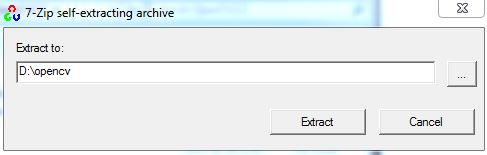
\includegraphics[scale=0.8]{img/user/unpack}
	\caption{Extract Opencv}
\end{figure}

\item{Set the OpenCV environment variable and add it to the systems path}\\

Add the folder containing the dynamic libraries to your system path. If using Visual Studio 2013, it will be 
$<$opencv\_install\_path$>$ $\backslash$ build $\backslash$ x86 $\backslash$ vc12 $\backslash$ bin;\\

For 64-bit Operating Systems: Visual Studio generates 32-bit code by default, so unless you have
downloaded the 64-bit compilers separately, you should still use the x86 versions of the libraries. For those steps, use the method below:\\

\begin{figure}[!h]
\centering
\begin{subfigure}{.5\textwidth}
  \centering
  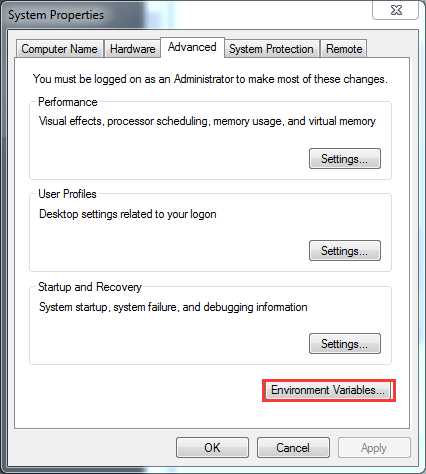
\includegraphics[scale=0.5]{img/user/system}
  \caption{System Properties and Environment Variable}
  \label{fig:sub1}
\end{subfigure}%
\begin{subfigure}{.5\textwidth}
  \centering
  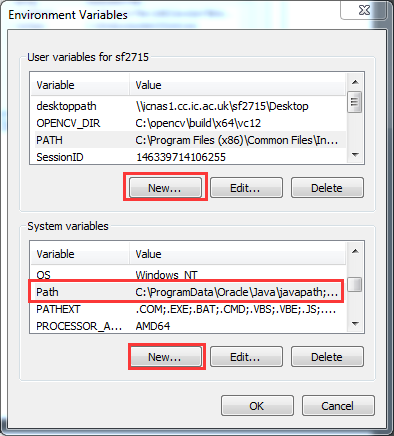
\includegraphics[scale =0.5]{img/user/variable}
  \caption{Choose New Variable and system path}
  \label{fig:sub2}
\end{subfigure}
\begin{subfigure}{.5\textwidth}
  \centering
  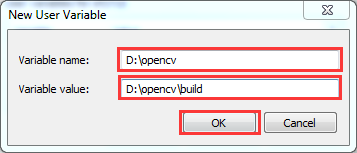
\includegraphics[scale=0.5]{img/user/newr}
  \caption{Enter name: OpenCV\_DIR and hit OK}
  \label{fig:sub1}
\end{subfigure}%
\begin{subfigure}{.5\textwidth}
  \centering
  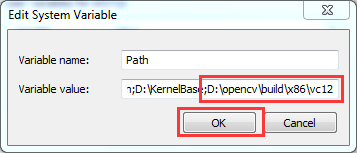
\includegraphics[scale =0.5]{img/user/newr2}
  \caption{Add the appropriate path to the END of the value}
  \label{fig:sub2}
\end{subfigure}
\caption{Choose New Variable and Setting system path}
\label{fig:test}
\end{figure}

\newpage
\item{Another way is to build from source: Configuration with CMake}\\

For anything more complex than the basic stuff, we need to build from scratch. Open CMake \cite{cmake} and point it at the $<$opencv\_install\_path$>$. Choose a build directory. Anywhere except build is fine. Select the IDE version and hit finish. Here we choose Visual Studio 12. Note: in case you can choose between different compilers for making either 32 bit or 64 bit libraries. CMake will start out and based on the system variables to automatically locate as many packages as possible. \\

\begin{figure}[!h]
\centering
\begin{subfigure}{.55\textwidth}
  \centering
  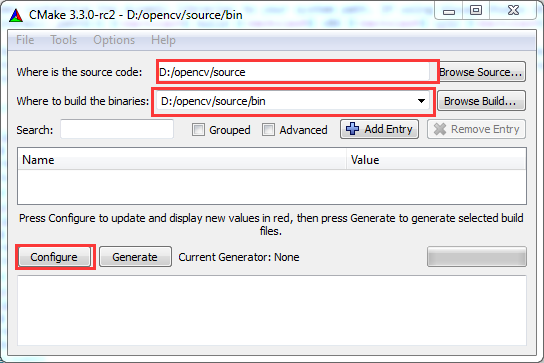
\includegraphics[scale=0.4]{img/user/cmake}
  \caption{Configure Opencv}
  \label{fig:sub1}
\end{subfigure}%
\begin{subfigure}{.3\textwidth}
  \centering
  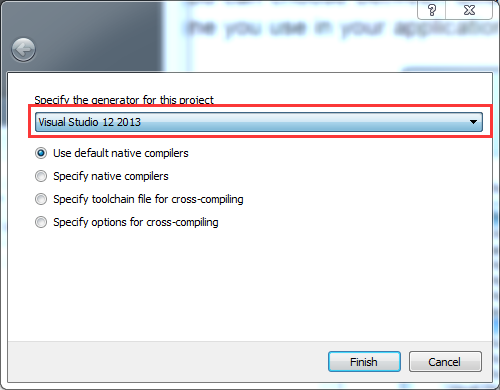
\includegraphics[scale =0.4]{img/user/configure}
  \caption{Select the IDE version}
  \label{fig:sub2}
\end{subfigure}
\caption{Configure OpenCV}
\label{fig:test}
\end{figure}


Figure A.4 shows selecting any extra features you need, then providing any extra info to make the red lines go away. \\

\begin{figure}[!htb]
	\centering
	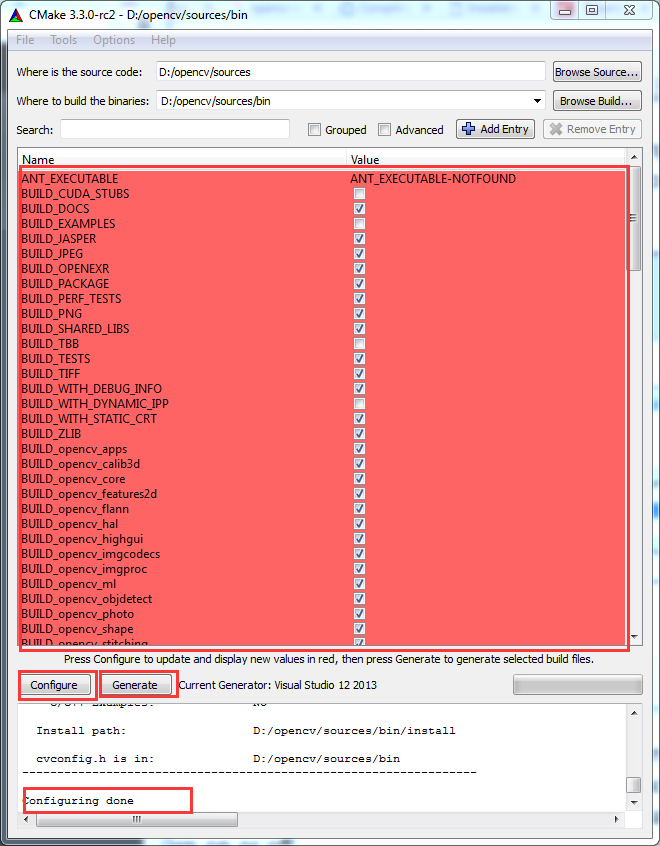
\includegraphics[scale=0.55]{img/user/select}
	\caption{Extract Opencv}
\end{figure}

After configuration, in the bin folder, double click OpenCV.sln (Open with Visual Studio 2013). Go to ALL\_BUILD in the Solutions Explorer window, right click on it and choose Build. This will create all the lib and dll files for debugging. Note: you need change Debug to Release, and compile. Then right clicked on INSTALL under CMakeTargets for both Debug and Release. This combines all the lib and dll files into a single “lib” and a single “bin” folder. And then setting the system path like previous step.

\item{Setting the Visual Studio}
Right Click the solution to properties. Go the C++ groups General entry and under the “Additional Include Directories” add the path to your OpenCV include ((OPENCV\_DIR) $\backslash$.. $\backslash$.. $\backslash$include)\\

Next go to the Linker - General and under the “Additional Library Directories” add the libs directory ((OPENCV\_DIR) $\backslash$ lib), including lib, bin, and stalib. Then go to the Linker-Input and under the “Additional Dependencies” entry add the name of all modules which you need to use. After that, you could compile this project.\\

\begin{figure}[!htb]
	\centering
	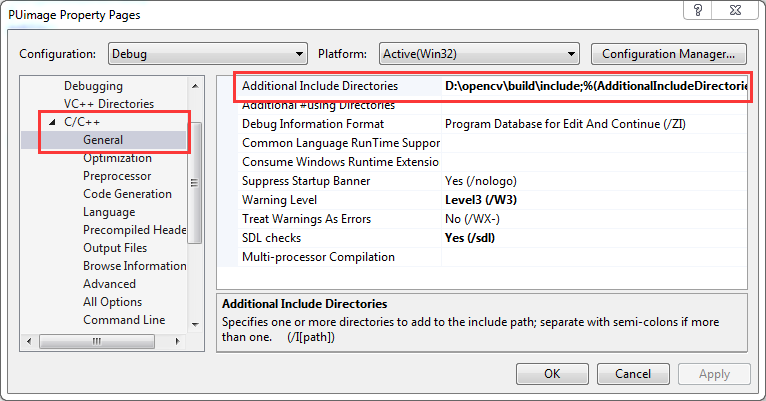
\includegraphics[scale=0.45]{img/user/Clink}
	\caption{C++ Additional Include Directories}
\end{figure}

\begin{figure}[!htb]
	\centering
	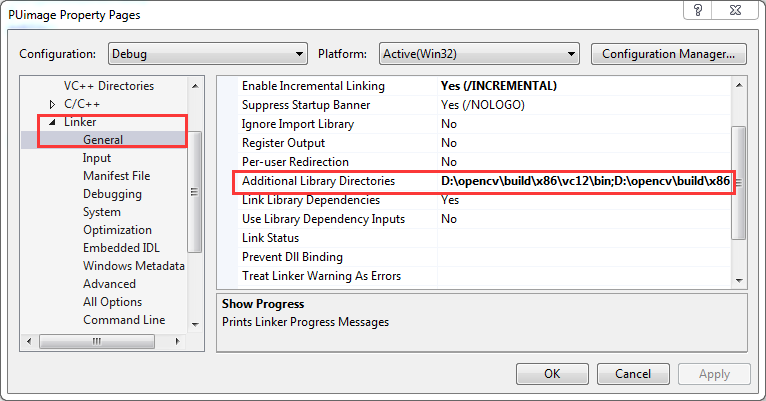
\includegraphics[scale=0.45]{img/user/linker}
	\caption{Linker Additional Library Directories}
\end{figure}

\begin{figure}[!htb]
	\centering
	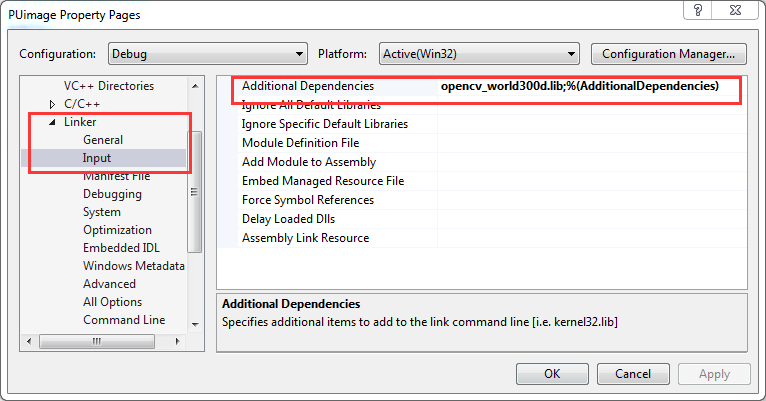
\includegraphics[scale=0.45]{img/user/input}
	\caption{Linker Additional Library Directories}
\end{figure}

\end{enumerate}

\newpage
\section{Software Dependencies}
\begin{itemize}
\item{Visual Studio 2013}
\item{MFC Desktop Applications}
\item{OpenCV 3.0}
\item{CMake 3.3.0}
\end{itemize}